\documentclass[12pt,a4paper]{article}

\input{style.sty}

%% metadata for pdf 
\newcommand{\pdfsubj}{COMP3301\slash COMP7308}
\newcommand{\pdftitle}{Assignment 2 --- Encrypting device driver}
\newcommand{\pdfauthor}{John Williams and Sam Kingston}
\newcommand{\assignnum}{a2}
\newcommand{\assignweight}{20\% }
\input{hypersetup.tex}

%% released 16 September 2011
\newcommand{\duedate}{8pm Thursday 6 October 2011}

%% end of preamble

\begin{document}

\input{title.tex}

\begin{center}
Version 1.0 --- 16 September 2011
\end{center}

\subsection*{Introduction}

The goal of this assignment is to give you practical experience writing a
device driver for Linux, and to learn how kernel modules are a useful and
powerful way of implementing operating systems concepts.

It is highly recommended you complete the two practicals surrounding this
assignment (Hello kernel world and character device drivers) before attempting
this assignment.

\input{plag.tex}

\subsection*{Overview}

The assignment is to create a Linux device driver interface to an encryption
coprocessor. Since we do not have special encryption hardware, the driver will
also perform the cryptography computations. The encryption/decryption algorithm
is a simple XOR-based stream cipher (details are given below).

The architecture of the driver is as follows:

\begin{compactitem}
    \item The device node is located at \texttt{/dev/crypto}.
    \item After opening the device, processes use \texttt{ioctl()} calls to
    create or attach to one or more encryption buffers, and to set the
    encryption key.
    \item Once a file descriptor is attached to a buffer, \texttt{read()} and
    \texttt{write()} operations are used to send and receive
    plaintext\slash ciphertext to and from the device.
    \item The \texttt{mmap()} operation is supported so that processes may inspect a buffer's contents directly.
    \item After completing the cryptography operations, the process detaches from
    and\slash or destroys the buffers using \texttt{ioctl()} calls, before finally
    closing the file descriptor.
\end{compactitem}

\subsection*{Device registration}

When loaded, your device driver must register itself with major number 250 using
the dynamic allocation method described in the Linux Device Drivers, 3rd
edition book, chapter 3. The minor number should be automatically assigned by
the kernel. \textbf{Do not} use the ``older way'' (\texttt{register\_chrdev()})
--- you will lose marks if you do.

After registration, your driver must print out its assigned major and minor
number to the kernel's ring buffer in the following format (\texttt{KERN\_INFO}
is sufficient):

\texttt{crypto: major=MAJOR, minor=MINOR}

(where \texttt{MAJOR} is the assigned major number and \texttt{MINOR} is the
assigned minor number.) For example:

\texttt{crypto: major=250, minor=0}

You should ensure when the driver is unloaded it unregisters itself and cleans
up any memory it had allocated during operation. Your driver should not leak
any memory.

\subsection*{File operations}

A skeleton \textit{fops} struct has been defined for you in \textit{fops.c} and
\textit{fops.h} (both available on the course website). You should use this as
a basis for writing your module. All of the callbacks in the structure need to
be implemented.

\subsection*{Buffers}

The device uses buffers internally to store the data received through a
\texttt{write(2)} system call. Initially, the device has no buffers allocated;
to use the device a process must make an ioctl call to create at least one
buffer (see below for details on all of the ioctl calls). 

Each buffer has a unique identifier represented by an unsigned integer.
Identifiers are to start at 1 and be incremented every time a new buffer is
created. Identifiers may be reused, however it is up to you to guarantee
uniqueness across all buffers that exist in the driver at any given time.

Before reading and writing to a buffer, a file descriptor must attach to it
through an ioctl call.

A buffer must be explicitly created but can be deleted in one of two ways:
either an explicit ioctl call to destroy the buffer, or when there are no file
descriptors remaining attached to the buffer. This means that you will need to
implement simple reference counting to ensure buffers are removed when the last
file descriptor detaches from it. This automatic deletion procedure should be
run whenever a buffer is detached from.

Due to this behaviour, when creating a buffer the driver should transparently
attach the file descriptor to that buffer, to prevent it from being removed
at the next removal point.

Each buffer has a fixed-size of 8,192 bytes (8K) and can be read and written to
independently of each other. This means that each buffer has two variables
associated with it: a read offset and a write offset, and has first-in,
first-out semantics. These `pointers' determine where the next read and write
calls (respectively) will operate from. Writing past the end of the buffer
should wrap around to the start, but attempting to write past the current read
pointer should fail with \texttt{-ENOBUFS}.

A buffer may have at most one reader and one writer attached to it at any given
time, which may be from the same file descriptor opened for both reading and
writing, or two file descriptors, one opened for reading and the other for
writing. Whether a file descriptor is a reader or writer (or both) is specified
by its \textit{user-space} access mode to \texttt{open(2)} (there are
complimentary definitions inside the kernel that match these modes, see the
\texttt{linux/fs.h} header file):

\begin{longtable}{l l}
    \toprule
    \textbf{\textit{User-space} access mode} & \textbf{Meaning} \\
    \midrule

    \texttt{O\_RDONLY} & reader \\
    \texttt{O\_WRONLY} & writer \\
    \texttt{O\_RDWR} & reader and writer \\

    \bottomrule
\end{longtable}

This restriction must be enforced when attempting to attach to a buffer, and an
error returned if there is already a reader or writer attached (depending on
the mode). More on this behaviour is described in the \texttt{ioctl.h} file.

\subsection*{Encryption}

Each open file descriptor must support a settable encryption mode. This mode
specifies to the driver when it should encrypt (and decrypt) data being passed
through it, and on which call (read\slash write). The mode can be specified
through the \texttt{CRYPTO\_IOCSMODE} ioctl call (specified below). This call
also allows the key to be set (which is used as the initialisation vector). You
may assume that during marking keys that fit into 8-bits (a \texttt{char}) will
be used. You do not have to handle the case of your driver being passed keys
larger than this size (though it is trivial to implement if you wish).

For instance a process may set its write calls to encrypt, and its read calls to
decrypt. This behaviour would assert that the driver is successfully encrypting
and decrypting the data given. Alternatively, the process may just set the mode
on one of the read\slash write operations, and leave the other unset (this assumes
it would not call the other operation).

The encryption algorithm to be used is an XOR-based stream cipher, given by the
following formulae:

Encryption: $C_i = P_i \oplus C_{(i-1)}$

Decryption: $P_i = C_i \oplus C_{(i-1)}$

\vspace{0.5cm}

(where $C$ is ciphertext, $P$ is plaintext, $C_{-1}$ is the key or initialisation vector and $\oplus$ is an 8-bit wide, bitwise XOR operator.)

\vspace{0.5cm}

For example, to encrypt the plaintext \texttt{0x1 0x12 0x2 0xF} with the key \texttt{0x3}:

(\textit{so} $IV = \texttt{0x3}$ \textit{and} $P = \texttt{0x1 0x12 0x2 0xF}$)

\vspace{0.5cm}

$C_0 = \texttt{0x1} \oplus \texttt{0x3} = \texttt{0x2}$

$C_1 = \texttt{0x12} \oplus \texttt{0x2} = \texttt{0x10}$

$C_2 = \texttt{0x2} \oplus \texttt{0x10} = \texttt{0x12}$

$C_3 = \texttt{0xF} \oplus \texttt{0x12} = \texttt{0x1D}$

\vspace{0.5cm}

Therefore $C = \texttt{0x2 0x10 0x12 9x1D}$. Decrypting it gets the same
plaintext back:

\vspace{0.5cm}

$P_0 = \texttt{0x2} \oplus \texttt{0x3} = \texttt{0x1}$

$P_1 = \texttt{0x10} \oplus \texttt{0x2} = \texttt{0x12}$

$P_2 = \texttt{0x12} \oplus \texttt{0x10} = \texttt{0x2}$

$P_3 = \texttt{0x1D} \oplus \texttt{0x12} = \texttt{0xF}$

\vspace{0.5cm}

Therefore $P = \texttt{0x1 0x12 0x2 0xF}$, which is the same as the original
plaintext given.

Note that the encryption key is only used for the initialisation vector (IV),
which is XORed with the first byte of the first \texttt{write()} call to a
buffer. Consecutive writes should continue the stream and use the last
ciphertext byte of the last write as their $C_{i-1}$.

\subsection*{Using the device}

You must implement the following file operations in the device driver:

\subsubsection*{open}

Opening the device will set up any data structures required to store the state for
this file descriptor.

\subsubsection*{close}

Closing the device will detach from a buffer (if one is attached to) and clean
up any memory used by that file descriptor. If the file descriptor was attached
to a buffer, and this was the final reference to that buffer, it should be
destroyed.

\subsubsection*{read}

A read call can only be made if the file descriptor is already attached to a
buffer. If it is, the driver must attempt to copy the requested bytes from the
buffer into the user-space process, applying whichever encryption mode is set
on the file descriptor. For instance, if the file is set to decrypt on read,
then all data being copied from the buffer should be decrypted, and the
plaintext is transferred to the process.

If the read mode has not been set at the time of the call, then the driver
should act as if it were set to passthrough, and return the raw data from the
buffer (regardless of whether or not it is encrypted).

\subsubsection*{write}

A write call can only be made if the file descriptor is already attached to a
buffer. If it is, the driver must attempt to copy the data given into the
attached buffer, applying whichever encryption mode is set on the file
descriptor. For instance, if the file is set to encrypt on write, then all data
being written to the buffer should be encrypted, and the ciphertext stored in the
buffer.

If the write mode has not been set at the time of the call, then the driver
should act is it it were set to passthrough, and place the raw data in the
buffer (regardless of whether or not it is encrypted).

\subsubsection*{mmap}

You must also implement an \texttt{mmap()} file operation in the device driver that
allows a user-space process to request a pointer into the buffer it is attached
to. If the file descriptor passed through the \texttt{mmap()} call is not
attached to a buffer, the driver should return \texttt{-EOPNOTSUPP}. Attempting to
map any size that is not page-aligned or a size greater than the maximum buffer
length is an error and the driver should return \texttt{-EIO}. This means that
the only valid mapping sizes that a process can request are 4K and 8K.

Otherwise, the driver must attempt to map the buffer into the user-space
process' virtual address space. If the user-space process requests a specific
offset this must be obeyed (providing it is page-aligned and does not exceed
the size of a buffer, or \texttt{-EIO} should be returned). If
\texttt{PROT\_WRITE} is \textbf{not} specified by the user-space program in the
protocol field, then a read-only mapping should be created. In this case, the
virtual memory area being mapped should be protected from writes so the
user-space process faults if it attempts to do this.

For the purposes of this assignment you may ignore the flags field to
\texttt{mmap(2)} and your device driver does not have to implement this.

\subsection*{ioctl calls}

The device driver is to be controlled through various ioctl calls. These are listed
below for reference. A more detailed description and examples on each ioctl is provided
in the \texttt{ioctl.h} file, available on the course website.

\begin{longtable}{l p{4cm} l p{4cm}}
    \toprule
    \textbf{ioctl} & \textbf{Description} & \textbf{Arguments} & \textbf{Returns} \\
    \midrule

    \texttt{CRYPTO\_IOCCREATE} & Creates a new buffer & None & Buffer id or error \\
    \texttt{CRYPTO\_IOCTDELETE} & Deletes an existing buffer & Buffer id & 0 on success or error \\
    \texttt{CRYPTO\_IOCTATTACH} & Attaches to an existing buffer & Buffer id & 0 on success or error \\
    \texttt{CRYPTO\_IOCDETACH} & Detaches from the already attached buffer & None & 0 on success or error \\
    \texttt{CRYPTO\_IOCSMODE} & Set the mode of subsequent read\slash write calls & \texttt{struct crypto\_smode *} & 0 on success or error \\

    \bottomrule
\end{longtable}

Note that the ioctl definitions have been defined for you in \texttt{ioctl.h}.
You should use this header file when creating your device driver and test
programs.  Please do not modify this file --- a clean copy will be used during
marking and any changes you have made will be discarded. If your implementation
relies on any changes made then you may fail some or all of the automated tests.

\subsection*{Return codes}

Each of the file operations and ioctl calls listed above must return one of the
following status codes (unless otherwise described):

\begin{longtable}{l l}
    \toprule
    \textbf{Value} & \textbf{Meaning} \\
    \midrule
    0 & Success \\
    \texttt{-ENOMEM} & Not enough memory to satisfy the request \\
    \texttt{-EINVAL} & An argument given was invalid \\
    \texttt{-EALREADY} & A file descriptor is already attached as a reader or writer \\
    \texttt{-EOPNOTSUPP} & The operation cannot occur when not attached to a buffer \\
    \texttt{-EIO} & \texttt{mmap()} size is not page-aligned or has an invalid size \\
    \bottomrule
\end{longtable}

\subsection*{Test program}

As part of the assignment, you must create a test program (written in C) that
demonstrates your implementation of the device driver. The test program should
be placed in a \textit{a2/test} sub-directory in your repository with a
Makefile that can produce the binary specified below. Your test program will be
tested against both your implementation of the device driver, and a reference
implementation. The test program does not test the entire driver specification
--- it will be run through a test harness.

The test program shall be called \texttt{echat} and is a simple chat program
that uses an encrypted IPC pipe (via the encrypted device created in the
assignment). Since it is modelled on a pipe, it can only have two chat users.
Both will open the test program on the same machine, but with different
arguments.  The first chat user will open the program with one argument (this
will create the buffers required for chatting) and the second chat user will
open the program with three arguments (which will attach to the buffers
specified).  You do not have to handle the case where no arguments are given,
or more than three arguments are given.

You should ensure that you only open the device with the mode required for each
file descriptor. No file descriptor in the test program should have the device open
for both reading and writing at once.

You may assume that the device exists at \texttt{/dev/crypto} and you may hardcode
this into your test program.

\subsubsection*{First chat user}

\texttt{Usage: echat encryption\_key}

When run with a single argument, the program should open the device twice (once
for reading, once for writing) and create two buffers, one for each file
descriptor (we will call these the first buffer and the second buffer). The buffer
identifiers should be printed on standard error in the following format:

\texttt{first\_buffer\_id: X, second\_buffer\_id: Y}

(where \texttt{X} and \texttt{Y} are the respective identifiers.)

The first buffer is used for text being sent from the first user to the second
user, and the second buffer is used for text being sent from the second user to
the first user.

\begin{figure}[h]
    \centering
    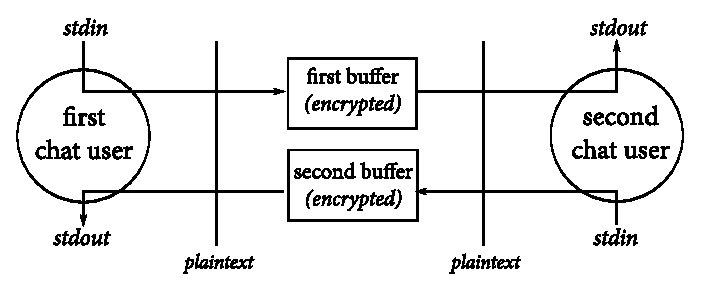
\includegraphics{echat.eps}
    \label{fig:echat}
\end{figure}

The encryption mode should be set accordingly as per the argument given and the
read\slash write direction required. You may assume the encryption key is given
as a string representation of an 8-bit hexadecimal value (for example
\texttt{"0x3"}). You do not have to handle the case where the key is not given
in this format.

After setting up the buffers, the program should wait for inputs as per the
\textit{Chat behaviour} section, below.

\subsubsection*{Second chat user}

\texttt{Usage: echat encryption\_key first\_buffer\_id second\_buffer\_id}

When run with three arguments, the program acts as the second chat user and
attaches to the buffers given. After attaching to the buffers, the program
should wait for inputs as per the \textit{Chat behaviour} section, below.

\subsubsection*{Chat behaviour}

The program should spawn two threads (using pthreads) and wait for input lines
(terminated by a newline) on both standard in and the user's respective
directional buffer (read from the first buffer for the second chat user; read
from the second buffer for the first chat user).

When an input line is read on standard in, it should be written to the other
buffer (write to the second buffer for the second chat user; write to the first
buffer for the first chat user).

When an input line is read from the respective directional buffer (see above),
it should be printed to standard out.

You should be able to type text in the first invocation of the program and
have it appear on standard out of the second invocation, and vice versa.

You do not have to handle the case where one chat user detaches while the other
is still attached.

\subsubsection*{End-of-file handling}

If an end-of-file (EOF) condition is detected, your program should close the
device and exit with status 0 (make sure you handle this case as the test
script may rely on it). An end-of-file condition is detectable by the read
system call returning 0 (which will in turn cause \texttt{fgets(3)} to return
\texttt{NULL}, if you are using it). This occurs when there is no more input
available from the given input stream (for instance, standard in). You can test
this in \texttt{echat} by typing \verb|^D| in a terminal (Control + D). This
will cause your program to read EOF from standard in and it should exit as
specified. If standard in is redirected from a file, the same behaviour should
occur.

\subsection*{Tips}

\begin{compactitem}
    \item The driver must not leak memory while running, and must clean up all
        memory used when unloaded.
    \item It is recommended you split your implementation across multiple
        C source files.
    \item Be aware of allocating large local variables or buffers. You are operating
        in the kernel and have very limited stack space available to you.
    \item A linked-list may be useful in representing the buffers in the
        kernel. An implementation has been provided on the course website that you
        are free to use (at your own risk: it is not guaranteed to be bug-free!)
\end{compactitem}

\subsection*{Short-response questions}

\begin{enumerate}
    \item Why are ioctl calls required as opposed to implementing their
    functionality in read\slash write functions?

    \item What is the difference between using \texttt{kmalloc} and
    \texttt{vmalloc} in kernel land? How would this effect your device
    driver? Justify your answer with regards to your implementation and how it
    would differ if you changed from \texttt{kmalloc} to \texttt{vmalloc}
    (or vice versa).

    \item Discuss the effects of \texttt{fork} and the \texttt{dup} family
    of system calls on your device driver. Some things to consider are what
    happens to buffer reference counting, whether or not the two processes
    share the same attached buffer, what happens when one closes the device,
    \textit{etc.} You may wish to write a program that does this and use its
    behaviour to justify your answer (you do not need to submit any program
    written for this question).

    \item Assume you have access to a DMA-capable hardware encryption device
    that your driver may use to perform the cryptography computations. What
    steps would you need to take in your driver to use this hardware device?
    What things do you have to consider when making DMA requests to the device?
    Sketch out what a read and a write call would look like from the
    perspective of your device driver (pseudocode is fine, but must be detailed
    enough to easily convert to a higher-level language such as C).
\end{enumerate}

\subsection*{Code compilation}

Your implementation must compile as a Linux kernel module (with a \texttt{.ko}
extension). It must compile and be loadable on the version of the virtual image
provided on the website. See the kernel module practical for information on
Makefiles for kernel modules.

Your module will be built by running the following in the \texttt{a2}
repository directory:

\texttt{make}

The test program will be built by entering into the \textit{a2/test}
subdirectory and running:

\texttt{make}

You should ensure that the \texttt{echat} binary is created with the
\texttt{-Wall -std=gnu99} compiler flags.

\input{coding-style.tex}

\input{groupwork.tex}

\input{submission.tex}

\clearpage
\subsection*{Assessment Criteria}

Marks will be awarded based on the modified scheduling behaviour and the coding
style used, as well as your responses to the questions above.

\subsubsection*{Functionality (70 marks)}

\begin{longtable}{p{13cm} r}
    \toprule
    \textbf{Criteria} & \textbf{Marks available} \\
    \midrule

    \textbf{Kernel module} & \textbf{3 marks} \\
    Module registers itself as a character device using the dynamic method when loaded and prints its major and minor numbers in the correct format & 1 \\
    Module unregisters itself as a character device when unloaded & 1 \\
    Module will not unload while a file descriptor is open in the device & 1 \\

    & \\
    \midrule
    \textbf{Opening and closing} & \textbf{2 marks} \\
    Device can be opened and closed by a single file descriptor & 1 \\
    Device can be opened and closed by multiple file descriptors and processes & 1 \\

    & \\
    \midrule
    \textbf{Buffer creation} & \textbf{7 marks} \\
    A single buffer can be created through an ioctl call & 1 \\
    Multiple buffers can be created through consecutive ioctl calls by a single file descriptor & 1 \\
    Multiple buffers can be created through consecutive ioctl calls by multiple file descriptors & 2 \\
    File descriptor is attached to the buffer when a create call is issued & 1 \\
    Buffer identifier allocation scheme ensures uniqueness & 1 \\
    Arbitrary number of buffers can be created (up to $\texttt{INT\_MAX}-1$) & 1 \\

    & \\
    \midrule
    \textbf{Buffer destruction} & \textbf{3 marks} \\
    A single buffer can be destroyed through an ioctl call & 1 \\
    Reference counting destroys a buffer when no file descriptors are attached to it anymore & 1 \\
    Correct error code is returned when attempting to explicitly destroy a buffer that has a positive reference count & 1 \\

    & \\
    \midrule
    \textbf{Attaching and detaching to buffers} & \textbf{6 marks} \\
    A single file descriptor can attach to a buffer & 1 \\
    Multiple file descriptors can be attached to a single buffer at the same time & 1 \\
    Correct error code returned when attempting to attach to a buffer when already attached to another & 1 \\
    Correct error code returned when attempting to attach to a non-existent buffer & 1 \\
    Correct error code returned if a reader or writer already is attached to a buffer & 2 \\

    & \\
    \midrule
    \textbf{Encryption} & \textbf{13 marks} \\
    Encryption mode set to encrypt on write stores correct ciphertext in buffer & 5 \\
    Encryption mode set to decrypt on read returns correct plaintext in userspace & 5 \\
    Encryption mode set to passthrough on reading and writing yields the same data & 3 \\

    & \\
    \midrule
    \textbf{Reading and writing to buffer} & \textbf{6 marks} \\
    Writing blocks of data (with any encryption mode) under the maximum buffer size succeeds & 1 \\
    Reading the same data as above (with any encryption mode) yields the input given & 1 \\
    Writing more then the maximum buffer size wraps around to start of buffer as specified & 3 \\
    Attempting to write past the read pointer fails as specified & 1 \\

    & \\
    \midrule
    \textbf{\texttt{mmap()}} & \textbf{10 marks} \\
    Mapping the size of a single page succeeds (regardless of requested length) & 3 \\
    Mapping the requested length (including when it covers multiple pages) succeeds & 2 \\
    Requesting a read-only mapping protects the address space from being written to & 2 \\
    Error is returned when not attached to a buffer & 1 \\
    Error is returned if length is invalid & 1 \\
    Error is returned if offset is invalid & 1 \\

    & \\
    \midrule
    \textbf{Test program --- \texttt{echat}} & \textbf{20 marks} \\
    Program opens the device correctly for each chat user with correct number of arguments & 2 \\
    First chat user creates buffers and prints out their identifiers as specified to standard error & 3 \\
    Second chat user attaches to buffers given & 1 \\
    Both chat users set the encryption mode and direction appropriately with given encryption key & 2 \\
    Program spawns two threads so not to block reading from both standard in and buffer & 3 \\
    Input read from standard in is written to the correct buffer from both directions & 4 \\
    Output from the correct buffer is written to standard out from both directions & 4 \\
    EOF is handled from standard in as specified & 1 \\

    \bottomrule
\end{longtable}

\subsubsection*{Documentation, style and build system (10 marks)}

\begin{longtable}{p{13cm} r}
    \toprule
    \textbf{Criteria} & \textbf{Marks available} \\

    \midrule
    Program builds cleanly with no compiler warnings (1 mark will be
        deducted per warning up to a maximum of 3) & 3 \\
    Comments throughout code where appropriate for the marker to understand & 2 \\
    Coding style follows the Linux kernel coding style document (1 mark will be
        deducted per violation up to a maximum of 3) & 3 \\
    Evidence of regular progress through Subversion commit history & 2 \\

    \bottomrule
\end{longtable}

\subsubsection*{Short-response questions (20 marks)}

Your responses will be assessed for their clarity and completeness, and marks
will be assigned as follows:

\begin{longtable}{p{13cm} r}
    \toprule
    \textbf{Question} & \textbf{Marks available} \\
    \midrule

    ioctl \textit{vs.} read\slash write functions & 3 \\
    \texttt{kmalloc} \textit{vs.} \texttt{vmalloc} & 3 \\
    Effects of \texttt{fork} and \texttt{dup} family of system calls & 6 \\
    Using a DMA-capable hardware encryption device & 8 \\

    \bottomrule
\end{longtable}

\end{document}
